\documentclass{beamer}
\usetheme{Madrid}

\usepackage{amsmath, amssymb, amsthm}
\usepackage{graphicx}
\usepackage{gensymb}
\usepackage[utf8]{inputenc}
\usepackage{hyperref}
\usepackage{tikz}


\title{1.6.27 Matgeo}
\author{AI25BTECH11012 - Garige Unnathi}
\date{}

\begin{document}

\frame{\titlepage}

% Question frame
\begin{frame}
\frametitle{Question}
Prove that the three points \textbf{A} (-4,6,10) , \textbf{B} (2,4,6) and \textbf{C} (14,0,-2) are collinear.
\\\end{frame}




% Solution steps
\begin{frame}
\frametitle{Solution}
 If ABC are collinear , then the matrix should have rank 1.
 \begin{align*}
{(\textbf{B} - \textbf{A} \quad \textbf{C} - \textbf{A})}^T
\end{align*}
\begin{align}
    {(\textbf{B} - \textbf{A} \quad \textbf{C} - \textbf{A})}^T =  
    \begin{bmatrix}
      6 & -2 & -4 \\
      18 & -6 & -12   
    \end{bmatrix}
\end{align}

\begin{align}
    R_2 = R_2 - 3R_1
\end{align}


\begin{align}
 \begin{bmatrix}    
6 & -2 & -4 \\
0 & 0 & 0 
\end{bmatrix}
\end{align}

 \end{frame}





% Graphical representation
\begin{frame}
Since all the elements of $R_2$ are zero, the rank of the matrix is one.

Hence ABC are collinear points.

\frametitle{Graphical Representation}
\begin{center}
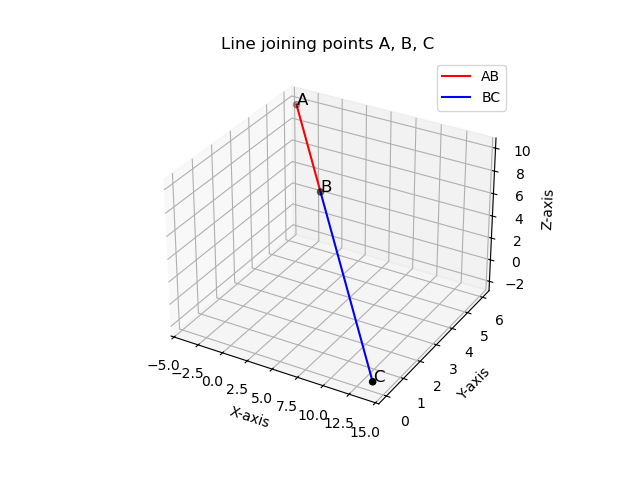
\includegraphics[width=0.6\linewidth]{/Users/unnathi/Documents/ee1030-2025/ai25btech11012/matgeo/1.6.27/figs/figs.png}
\end{center}
\end{frame}

\end{document}
